\section{Bridge - Step 5 EXTRA}
The next part of the program covered implementing a bridge into the program. The bridge only allows a certain number of cars to enter at any point in time, regardless of direction. \textbf{\textit{This part of the assignment is considered an extra expansion, and as such will not be present in later versions of the program.}}

The bridge itself follows a fairly simple implementation. 

When initialized, the bridge allows 6 cars to pass through. Note that it is not possible to turn off the bridge, merely to not show it. 

Below is the code run when a car tries to enter the bridge
\begin{lstlisting}
    public synchronized void enter() throws Exception {
        while(this.onBridge >= this.limit) wait();
        this.onBridge++;
    }
\end{lstlisting}

If a car tries to enter the bridge when the bridge has reached its limit, it will wait in a condition queue. If, however, the amount of cars on the bridge is less than the limit, the car is allowed to pass and the car count gets incrememnted. When a car leaves the bridge, the car counter gets decremented and a \texttt{notify} is sent out. If the bridge limit is changed, the variable simply gets set and a \texttt{notifyAll} is run to give waiting cars a chance to re-check if they can enter. All of the bridge methods are synchronized, as to guarantee mutual exclusion.

This impementation seeks to follow the invariant:
\begin{gather*}
    C \triangleq \forall \square \left( \texttt{onBridge} \leq \texttt{limit} \right)
\end{gather*}

That is; the amount of cars on the bridge will always be less than or equal to the amount of cars allowed to be on the bridge. This can of course be violated if we were to change the limit to an amount of cars currently on the bridge in a snapshot. Such a situation cannot, however, be accounted for with the invariant. Left to its own devices, the program will always uphold this invariant, and as such can be deemed correct. If the limit was to be changed such that \texttt{onBridge} \textgreater \; \texttt{limit}, the cars will simply be allowed to leave as normal, but no new cars will be allowed entry until \texttt{onBridge} \textless \;  \texttt{limit}. Upholding the invariant, however, can lead to deadlock. Since the bottom four cars (5, 6, 7 and 8) wait on the bridge before going into the alley, it is possible for them to block the top four cars (1, 2, 3 and 4) from exiting the alley, so as to not violate the invariant. An example of this can be seen in the picture below.

\begin{figure}[H]
    \centering
    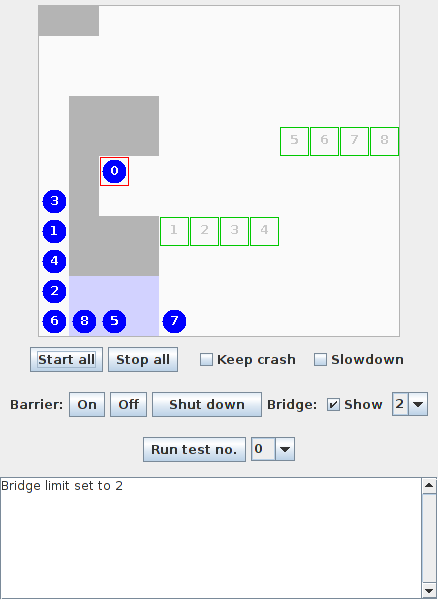
\includegraphics[scale=.4]{Step5/bridge_deadlock.png}
    \caption{A deadlock occuring on the bridge when the amount of cars allowed onto the bridge is 2. This deadlock could be resolved by raising the amount of cars allowed onto the bridge, thus allowing the cars from the alley to pass through.}
    \label{fig:bridge_deadlock}
\end{figure}

One possible fix to this is to extend the alley to include the bridge as well. This would make the bottom four cars stop and wait before the bridge, instead of on the bridge, thus allowing the top four cars to pass through. The limit of cars on the bridge would thus only serve to stop cars coming from the same direction to enter too quickly.  

We tested the bridge by setting the limit to various values, and checking if the limit was upheld. This proved to be true, regardless of what speed the cars ran at. Some limits, namely 2 and 3, would lead to the program reaching a deadlock. These could, however, be resolved by raising the limit on the bridge to allow new cars to enter, thus clearing them from the alley.


%Implementing the bridge into the main program

%\begin{itemize}
%    \item How was the bridge implemented?
%    \item Which situations allow for a deadlock to occur, and what could be done to prevent this? (in accordance to the limit values at which they may occur)
%\end{itemize}